\section{FUSE}
Filesystem in Userspace (FUSE) is a library that provides an interface to create filesystems in userspace rather than in kernel space which is otherwise often considered the standard when writing commercial filesystems\,\cite{Libfuse2021}. The reason to implement a filesystem in kernel space is that it leads to faster system calls than when writing a filesystem in userspace. However, while filesystems written with FUSE are generally slower than a kernel-based filesystem, using FUSE simplifies the process of creating filesystems. macFUSE is a port of FUSE that operates on Apple's macOS operating system and it extends the FUSE API\,\cite{HomeMacFUSE}. macFUSE provides an API for C and Objective C.

\begin{figure}[!ht]
	\begin{center}
	  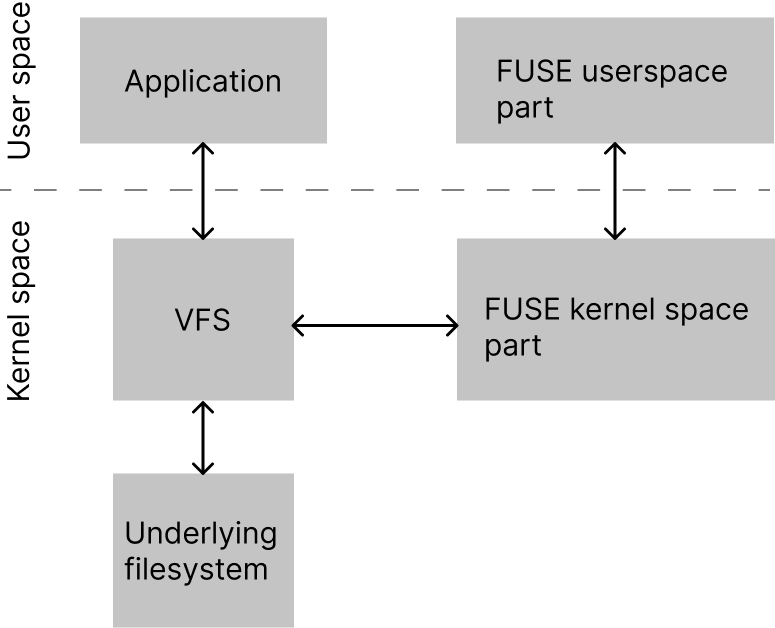
\includegraphics[width=0.5\textwidth]{figures/fuse_description.png}
	\end{center}
	\caption{Simple visualization of how FUSE operations are executed}
	\label{fig:fuse_desc}
\end{figure}

Figure~\ref{fig:fuse_desc} shows an overview how FUSE works. FUSE consists of a kernel space part and an userspace part that perform different tasks\,\cite{vangoorFUSENotFUSE2017}. The kernel part of FUSE operates with the Virtual Filesystem (\gls{VFS}) which is a layer in both the Linux kernel and the macOS kernel that exposes a filesystem interface for userspace applications\,\cite{goochOverviewLinuxVirtual, singhMacOSInternals2006}. The VFS interface is independent of the underlying filesystem and is an abstraction of the underlying filesystem operations which can be used on any filesystem the VFS supports. The userspace part of FUSE communicates with the kernel space part through a block device. Operations on a mounted FUSE filesystem are sent to the VFS from the user application, which is then sent to the kernel part of FUSE. If needed, the operations are transmitted to the userspace part of FUSE where the operation is handled and a response is sent back to the VFS and the user application through the FUSE kernel module. However, some actions can be handled by the FUSE kernel module directly, such as if the file is cached in the kernel part of FUSE\,\cite{vangoorFUSENotFUSE2017}. The response is then sent back to the user application from the kernel module through the VFS.